\documentclass[a4paper,12pt]{article}
\usepackage[T2A]{fontenc}
\usepackage[utf8]{inputenc}
\usepackage[english,russian]{babel}
\usepackage{circuitikz}
\usepackage{wrapfig}
\usepackage{makecell}

\usepackage{tabularx}
\usepackage{graphicx}

\usepackage{cancel}
\usepackage{amsmath,amsfonts,amssymb,amsthm,mathtools}
\usepackage{tikz}
\usetikzlibrary{intersections}
\usetikzlibrary{arrows.meta}
\usetikzlibrary{calc,angles,positioning}
\usepackage{float}
\graphicspath{ {C:/Users/George/Documents/MIPT_TEX/LAB_1_4_1} }



\begin{document}
	\begin{center}
		МОСКОВСКИЙ ФИЗИКО-ТЕХНИЧЕСКИЙ ИНСТИТУТ (НАЦИОНАЛЬНЫЙ ИССЛЕДОВАТЕЛЬСКИЙ УНИВЕРСИТЕТ) \\
		
		
		\hfill \break
		Факультет обшей и прикладной физики\\
		\vspace{2.5cm}
		\large{\textbf{Отчёт по лабораторной работе 1.4.1 <<Определение ускорения свободного падения с помощью колебаний физического маятника>>}}\\
		\hfill \break
		\\
	\end{center}
	
	\vspace{5cm}
	
	\begin{flushright}
		Выполнил:\\
		Студент гр. Б02-304\\
		Головинов. Г.А.
	\end{flushright}
	
	\vfill
	
	
	\begin{center} Долгопрудный, 2023 \end{center}
	
	\thispagestyle{empty}
	\newpage
	\pagenumbering{arabic}
	
	\section{Аннотация}
	\paragraph{Цель работы:} \hspace{-4mm} проверить справедливость формулы для периода колебаний физического маятника и \textbf{определить ускорение свободного падения}
	\paragraph{Используемые инструменты:} \hspace{-4mm} Физический маятник (стержень длиной $l=100$ см.) с возможностью изменения оси вращения, секундомер, весы.
	\section{Основные теоретические сведения}
	\begin{wrapfigure}{R}{0.3\textwidth}
		\vspace{0mm}
		\centering
		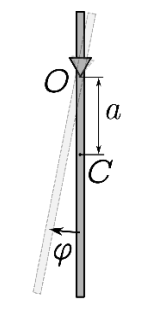
\includegraphics[width=0.7\linewidth,angle=-0.6]{pen.png} 
		\caption{Эксперементальная установка}
		\label{fig:1}
	\end{wrapfigure}
	Физический маятник -- твердое тело, способное совершать колебания в вертикальной плоскости, будучи подвешенным за одну из своих точек в полез силы тяжести. Ось качания (вращения) маятника можно изменять с помощью небольшой опорной призмы (см. рис. \ref{fig:1})
	\vspace{2mm}
	
	\noindent
	На рисунке показаны точки $O$ -- ось вращения маятника, $C$ -- центр масс стержня, $a$ -- расстояние между центром масс маятника и его осью вращения. 
	\vspace{2mm}
	
	\noindent
	Измерять период колебаний маятника будем с помощью секундомера, отчитывая время, за которое происходит ровно 10 полных колебаний. Погрешность измерения с помощью секундомера примем за $\sigma_t=0,3$ с, тогда для периода $\sigma'_t=0,03$ с. 
	\paragraph{Некоторые необходимые в работе уравнения}\mbox{}\\
	Момент импульса тела:
	\begin{equation}\label{eq:1}
		\centering
		L=J\omega
	\end{equation}
	где $J$ -- момент инерции тела (различается в зависимости от формы тела, для материальной точки определяется как $mr^2$),
	$\omega$ -- угловая скорость вращения тела.
	\begin{equation}\label{eq:2}
		\centering
		M=\frac{dL}{dt}
	\end{equation}
	где $M$ -- момент силы\\
	\noindent
	Подставляя \eqref{eq:1} в \eqref{eq:2} получим:
	\begin{equation}
		\label{eq:3}
		M=J\frac{d\omega}{dt}=J\varepsilon
	\end{equation}
	где $\varepsilon$ -- угловое ускорение.\\
	\noindent
	Для твёрдого тела справедливо
	\begin{equation}
		\label{eq:4}
		J=\sum_i{m_ir_i^2}
	\end{equation}\mbox{}\\
	\noindent
	Просуммировав (проинтегрировав) по всей длине стержня мы получим, что момент инерции $J_C$ относительно центра массы стержня равен
	\begin{equation}
		\label{eq:5}
		J_C=\frac{ml^2}{12}
	\end{equation}\mbox{}\\
	\noindent
	А по теореме \textit{Гюйгенса-Штейнера} момент инерции стержня относительно произвольной оси вращения равен
	\begin{equation}
		\label{eq:6}
		J=\frac{ml^2}{12}+ma^2
	\end{equation}
	где $a$ -- расстояние между центром масс стержня и осью вращения (см рис. \ref{fig:1})
	
	\paragraph{Стержень как физический маятник}
	
	При достаточно малых углах отклонения $\varphi$ момент возвращающей силы (тяжести) равен
	\begin{equation}
		\label{eq:7}
		M=-mga\sin{\varphi}\approx-mga\varphi
	\end{equation}
	при малых амплитудах колебаний они будут иметь характер гармонических, то есть описываться по гармоническому закону (синуса, косинуса).\\
	\noindent
	Период колебаний произвольного физического маятника с моментом инерции $J$, массой $m$, расстоянием между центром масс и осью вращения $a$ вычисляется по формуле
	\begin{equation}
		\label{eq:8}
		T=2\pi\sqrt{\frac{J}{mga}}
	\end{equation}
	такая формула получается через аналогию с пружинным маятником и формулой для него: $T=2\pi\sqrt{m/k}$, однако роль массы в данном случае играет момент инерции тела $J$, а жесткость $k$ -- коэффициент пропорциональности между моментом силы и величиной отклонения $mga$\\
	\vspace{2mm}
	\noindent	Подставляя момент инерции из \eqref{eq:6} в \eqref{eq:8} получим конечную формулу для периода колебаний нашего стержня:
	\begin{equation}
		\label{eq:9}
		T=2\pi\sqrt{\frac{\frac{l^2}{12}+a^2}{ga}}
	\end{equation}
	заметим существенное различие с известной формулой Гюйгенса для математического маятника: $T=2\pi\sqrt{l/g}$. Для любого физического маятника можно определить $l_{\text{пр}}=a+l^2/(12a)$ -- это будет длина математического маятника с таким же периодом, что и у физического.\\
	\paragraph{Уравнение колебаний}
	\noindent
	Итак, колебания физического маятника можно описать гармоническим законом
	\begin{equation}
		\label{eq:10}
		\varphi(t)=A\sin({\omega t+\alpha})
	\end{equation} 
	где $A$ -- угловая амплитуда, $\omega$ -- циклическая частота, $\alpha$ -- начальная фаза колебаний.
	\[
		\omega = \frac{2\pi}{T}=\sqrt{\frac{mga}{J}}
	\]
	
	\paragraph{Затухание колебаний}
	Если маятник не идеален и существуют потери энергии в окружающую среду существует зависимость амплитуды колебаний от времени:
	\begin{equation}
		\label{eq:11}
		A(t)=A_0e^{-\gamma t}
	\end{equation}
	где $\gamma=dA/A$ -- декремент затухания\\
	\noindent В данной работе мы находили $\tau_{\text{зат}}=1/\gamma$ при уменьшении амплитуды в 2 раза, а не в $e$ раз.\\
	\noindent Также для затухающих колебаний есть безразмерная величина $Q$, называемая добротностью. Она вычисляется по формуле:
	\begin{equation}
		\label{eq:12}
		Q=\pi\frac{\tau_{\text{зат}}}{T}
	\end{equation}
	
	
	\section{Результаты измерений и обработка данных}
	\paragraph{Небольшое замечание по поводу методики получения и обработки данных}
	Для каждого значения $a$ -- расстояния от центра масс до оси вращения было проведено 3 измерения, для каждого измерения по формуле
	\[
	\sigma=\sqrt{\frac{1}{2}\sum_{i=1}^3 (T-\langle T \rangle)^2}
	\]
	была найдена погрешность. Учитывая $\sigma_t'$ конечная погрешность измерения вычисляется по формуле:
	\[
	\sigma_{\text{полн}}=\sqrt{\sigma^2+\sigma_t'^2}
	\]
	\vspace{-10mm}
	\begin{table}[H]
		\centering
		\caption{Результаты измерения периодов колебаний маятника и их погрешности, шаг $\Delta a = $ 2 см.}
		\vspace{2mm}
		\begin{tabular}{|c|c|c|c|c|c|c|c|}
			\hline
			$a$, см & $T_1$, с & $T_2$, с & $T_3$, с & $\langle T \rangle$, с & $\sigma_i$ & $\sigma_T$ & $\sigma_{\text{полн}}$ \\
			\hline
			10 & 1,938 & 1,938 & 1,940 & 1,939 & 0,001 & 0,030 & 0,030 \\
			\hline
			12 & 1,811 & 1,825 & 1,822 & 1,819 & 0,007 & 0,030 & 0,031 \\
			\hline
			14 & 1,728 & 1,732 & 1,726 & 1,729 & 0,003 & 0,030 & 0,030 \\
			\hline
			16 & 1,684 & 1,661 & 1,668 & 1,671 & 0,012 & 0,030 & 0,032 \\
			\hline
			18 & 1,630 & 1,637 & 1,587 & 1,618 & 0,027 & 0,030 & 0,040 \\
			\hline
			20 & 1,573 & 1,550 & 1,569 & 1,564 & 0,012 & 0,030 & 0,032 \\
			\hline
			22 & 1,540 & 1,547 & 1,539 & 1,542 & 0,004 & 0,030 & 0,030 \\
			\hline
			24 & 1,537 & 1,533 & 1,530 & 1,533 & 0,004 & 0,030 & 0,030 \\
			\hline
			26 & 1,518 & 1,516 & 1,523 & 1,519 & 0,004 & 0,030 & 0,030 \\
			\hline
			28 & 1,528 & 1,517 & 1,538 & 1,528 & 0,011 & 0,030 & 0,032 \\
			\hline
			30 & 1,532 & 1,538 & 1,532 & 1,534 & 0,003 & 0,030 & 0,030 \\
			\hline
			32 & 1,540 & 1,542 & 1,533 & 1,538 & 0,005 & 0,030 & 0,030 \\
			\hline
			34 & 1,558 & 1,539 & 1,538 & 1,545 & 0,011 & 0,030 & 0,032 \\
			\hline
			36 & 1,561 & 1,558 & 1,569 & 1,563 & 0,006 & 0,030 & 0,031 \\
			\hline
			38 & 1,578 & 1,565 & 1,571 & 1,571 & 0,007 & 0,030 & 0,031 \\
			\hline
			40 & 1,586 & 1,586 & 1,579 & 1,584 & 0,004 & 0,030 & 0,030 \\
			\hline
			42 & 1,589 & 1,591 & 1,609 & 1,596 & 0,011 & 0,030 & 0,032 \\
			\hline
			44 & 1,617 & 1,617 & 1,617 & 1,617 & 0,000 & 0,030 & 0,030 \\
			\hline
			46 & 1,631 & 1,631 & 1,631 & 1,631 & 0,000 & 0,030 & 0,030 \\
			\hline
			48 & 1,650 & 1,650 & 1,650 & 1,650 & 0,000 & 0,030 & 0,030 \\
			\hline
		\end{tabular}
	\end{table}

	\noindent
	Случайная погрешность измерений оказалась много меньше, чем системная. Мы ее всё-равно будем учитывать, потому что в некоторых измерениях она действительно влияет на результат, однако можно сказать, что случайная погрешность измерений намного меньше инструментальной.\\
	\noindent
	По формуле \eqref{eq:9} находим ускорение свободного падения $g$.
	Его погрешность будет вычисляться по формуле:
	\begin{equation}
		\label{eq:13}
		\sigma_g=g\sqrt{\left(2\frac{\sigma_l}{l}\right)^2+\left(2\frac{\sigma_T}{T}\right)^2+\left(3\frac{\sigma_a}{a}\right)^2}
	\end{equation}
	Где $\sigma_l$ примем за 2 см, а $\sigma_a$ за 0,5 см
	
	\begin{figure}[H]
		\centering
		\caption{Полученная зависимость периода $T$ и квадрата периода $T^2$ от расстояния $a$ между центром масс маятника и его осью вращения}
		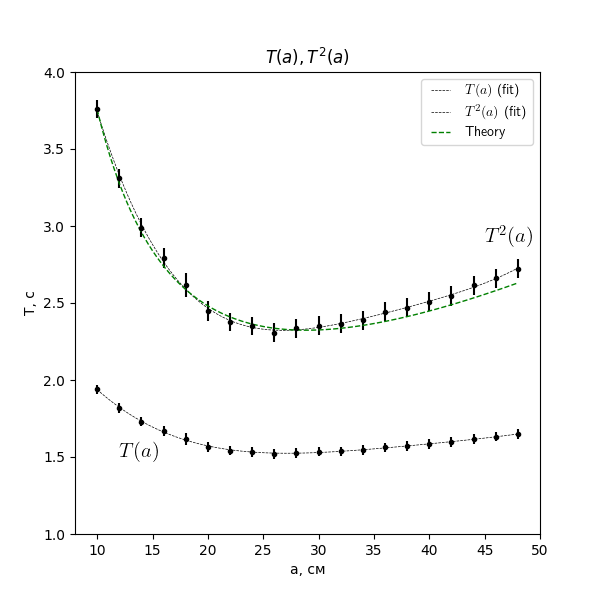
\includegraphics[width=0.9\linewidth]{fig2}
		\label{fig:fig2}
	\end{figure}
	
	\noindent
	Зелёным на графике показана теоретическая зависимость $T^2(a)$ по формуле \eqref{eq:9}\\
	
	\vspace{-5mm}
	
	\begin{table}[H]
		\centering
		\caption{Полученные значения $g$ и их погрешности}
		\vspace{2mm}
		\begin{tabular}{|c|c|c|c|c|c|c|c|c|}
			\hline
			$a$, см & $T$, c & $g$, $\frac{\text{м}}{\text{с}^2}$ & $\varepsilon_l$ & $\varepsilon_T$ & $\varepsilon_a$ & $\varepsilon_g$ & $\sigma_g$ & $|g-g_\text{теор}|$ \\
			\hline
			10 & 1,939 & 9,80 & 0,02 & 0,02 & 0,05 & 0,09 & 0,92 & 0,01 \\
			\hline
			12 & 1,819 & 9,71 & 0,02 & 0,02 & 0,04 & 0,08 & 0,79 & 0,10 \\
			\hline
			14 & 1,729 & 9,71 & 0,02 & 0,02 & 0,04 & 0,07 & 0,70 & 0,10 \\
			\hline
			16 & 1,671 & 9,63 & 0,02 & 0,02 & 0,03 & 0,07 & 0,64 & 0,18 \\
			\hline
			18 & 1,618 & 9,70 & 0,02 & 0,02 & 0,03 & 0,07 & 0,64 & 0,11 \\
			\hline
			20 & 1,564 & 9,95 & 0,02 & 0,02 & 0,03 & 0,06 & 0,59 & 0,14 \\
			\hline
			22 & 1,542 & 9,94 & 0,02 & 0,02 & 0,02 & 0,06 & 0,56 & 0,13 \\
			\hline
			24 & 1,533 & 9,86 & 0,02 & 0,02 & 0,02 & 0,05 & 0,53 & 0,05 \\
			\hline
			26 & 1,519 & 9,93 & 0,02 & 0,02 & 0,02 & 0,05 & 0,52 & 0,12 \\
			\hline
			28 & 1,528 & 9,77 & 0,02 & 0,02 & 0,02 & 0,05 & 0,50 & 0,04 \\
			\hline
			30 & 1,534 & 9,69 & 0,02 & 0,02 & 0,02 & 0,05 & 0,48 & 0,12 \\
			\hline
			32 & 1,538 & 9,68 & 0,02 & 0,02 & 0,02 & 0,05 & 0,47 & 0,13 \\
			\hline
			34 & 1,545 & 9,68 & 0,02 & 0,02 & 0,01 & 0,05 & 0,47 & 0,13 \\
			\hline
			36 & 1,563 & 9,56 & 0,02 & 0,02 & 0,01 & 0,05 & 0,44 & 0,25 \\
			\hline
			38 & 1,571 & 9,58 & 0,02 & 0,02 & 0,01 & 0,05 & 0,44 & 0,23 \\
			\hline
			40 & 1,584 & 9,58 & 0,02 & 0,02 & 0,01 & 0,04 & 0,43 & 0,23 \\
			\hline
			42 & 1,596 & 9,58 & 0,02 & 0,02 & 0,01 & 0,05 & 0,43 & 0,23 \\
			\hline
			44 & 1,617 & 9,50 & 0,02 & 0,02 & 0,01 & 0,04 & 0,41 & 0,31 \\
			\hline
			46 & 1,631 & 9,52 & 0,02 & 0,02 & 0,01 & 0,04 & 0,41 & 0,29 \\
			\hline
			48 & 1,650 & 9,48 & 0,02 & 0,02 & 0,01 & 0,04 & 0,40 & 0,33 \\
			\hline
		\end{tabular}
	\end{table}
	\noindent
	Заметим, что все полученные значения ускорения свободного падения $g$ оказались в пределах полученных нами погрешностей. Самое большое отклонение от табличных значений $\varepsilon_{max}$ составило $3,3\%$, а среднее $\varepsilon_{avg}$ -- лишь $1,6\%$
	
	\begin{figure}[H]
		\centering
		\caption{Зависимость $g(a)$ и сравнение полученных значений с табличными}
		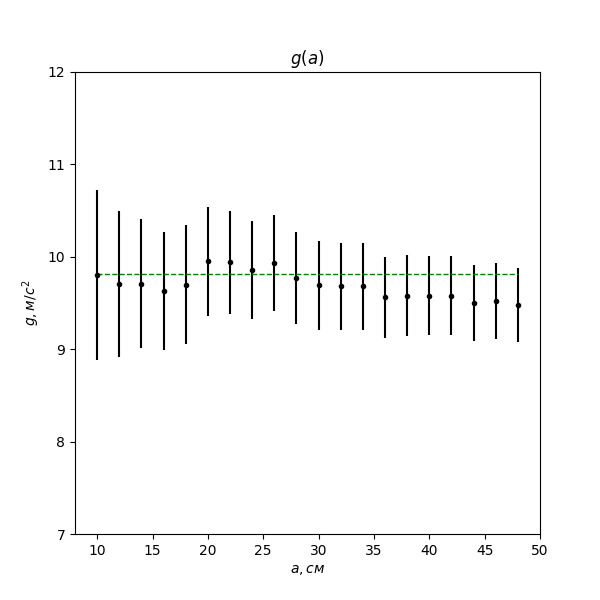
\includegraphics[width=0.9\linewidth]{fig3}
		\label{fig:fig3}
	\end{figure}
	
	
	\paragraph{Затухание колебаний}
	В результате измерений амплитуда колебаний уменьшилась в два раза примерно за $\tau_{\text{зат}}=$ 250 сек, что дает декремент затухания $\gamma \approx 0,004$. Добротность $Q$ получилась равной $\approx$ 500. Высокая добротность показывает, что потери при колебаниях намного меньше энергии вращательного движения и что в данной работе при $n =$ 10 полных колебаний их затухание не могло существенно повлиять на результаты.
	
	\subsection{Учёт влияния подвесной призмы}
	
	Для $a>30$ см заметно сильное отклонение от табличных значений. Это может быть объяснено тем, что в работе мы не учитывали движение призмы, которая выступает в качестве оси вращения для маятника. Учесть эту разницу можно с помощью соотношений:
	\begin{equation}
		\label{eq:14}
		x_c=\frac{m_\text{ст}a_\text{ст}-m_\text{пр}a_\text{пр}}{m_\text{ст}+m_\text{пр}}, \hspace{4mm} T=2\pi\sqrt{\frac{l^2/12+a^2}{g\left(1+\frac{m_\text{пр}}{m_\text{ст}}\right)x_c}}
	\end{equation}
		
	\vspace{5mm}
	\noindent
	Получим следующий результат:
	\begin{figure}[H]
		\centering
		\caption{Скорректированные значения $g(a)$ }
		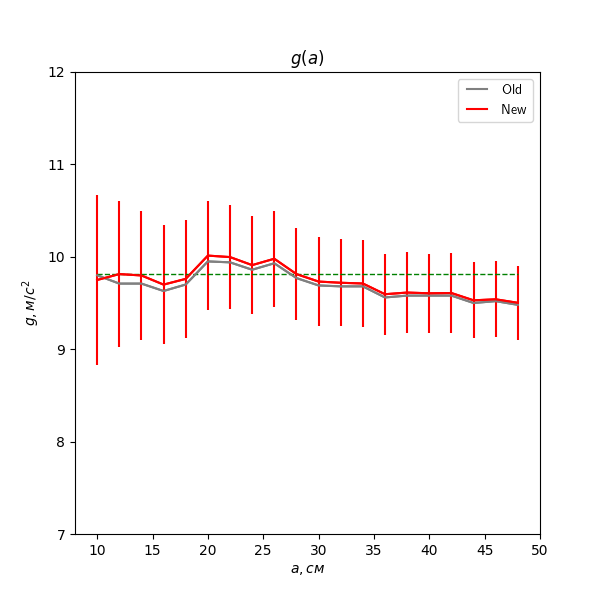
\includegraphics[width=0.9\linewidth]{fig4}
		\label{fig:fig4}
	\end{figure}
	\noindent
	Видно, что учёт призмы немного улучшил точность для небольших $a$, однако для $a>30$ см ситуация практически не изменилась. \\
	
	\noindent
	С новыми результатами для $g(a)$ с помощью метода $\chi^2$ находим итоговое значение ускорения свободного падения
	
	\begin{figure}[H]
		\centering
		\caption{Функционал $\chi^2$ для $g$}
		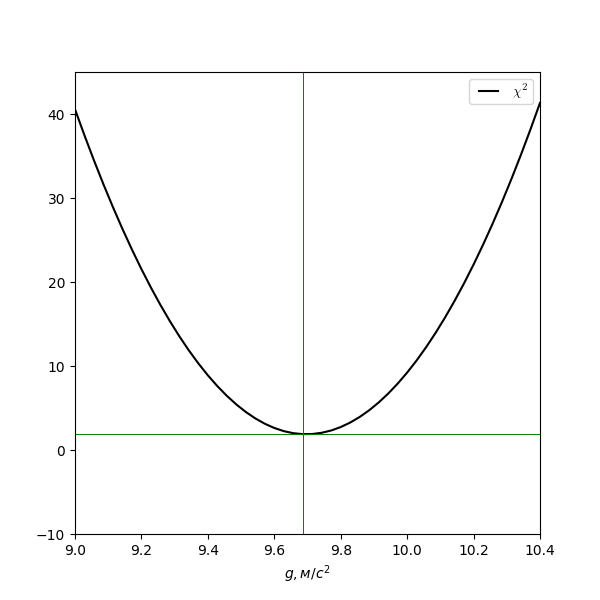
\includegraphics[width=0.9\linewidth]{fig5}
		\label{fig:fig5}
	\end{figure}
	
	\noindent
	Минимум функционала приходится на $g=9,6964$ $\text{м}/\text{с}^2$, при этом он равен $\chi^2_{\text{min}}\approx 1,88$. При $\chi^2=\chi^2_{\text{min}}+1$: $g=9,5844$ $\text{м}/\text{с}^2$, следовательно итоговая погрешность $\sigma_g=0,1121$ $\text{м}/\text{с}^2$
	
	\begin{equation}
		\label{eq:fin}
		g=(9,6964\pm 0,1121) \hspace{1mm} \text{м}/\text{с}^2
	\end{equation}
	
	\section{Обсуждение результатов и выводы}
	
	В ходе работы мы измерили ускорение свободного падения с помощью колебаний физического маятника. Полученные значения хорошо соотносятся с табличными (для отдельного измерения отклонение не больше $=3,3\%$).\\
	
	\noindent
	Табличное значение для московской широты $g\approx 9,8155$ $\text{м}/\text{с}^2$ находятся за пределами $\pm 1\sigma_g$, однако очень близко к этой границе. Итоговое отклонение от табличного значения составило $1,2\%$
	
	\paragraph{Учёт влияния подвесной призмы} Так как для $a>30$ см наблюдалось большое отклонение от табличных результатов, было принято решение учесть колебания подвесной призмы маятника. Это немного улучшило точность для небольших $a$, однако для $a>30$ см ситуация не изменилась. Это говорит о том, что отклонение обусловлено другими допущениями и <<неидеальностью>> установки и эксперимента. (Например: влияние затухания колебаний, неоднородность стержня и т.д.)\\
	\vspace{2mm}
	
	\paragraph{Другие выводы}
	\noindent
	Несмотря на это все полученные значения $g$ достаточно близки к табличным и почти попадают в пределы $\pm1\sigma$. Самый большой вклад в погрешность измерений внес неточный способ определения периода колебаний маятника (вообще сложно оценить погрешность измерений обычным секундомером <<на глаз>>), на самом деле она может быть как больше использованной нами, так и меньше. Кроме того, полученные зависимости $T(a)$ и $T^2(a)$ хорошо соотносятся с теорией (уравнения \eqref{eq:9} и \eqref{eq:14})
	
	
\end{document}